\subsection{Experimental Results}

Once the flights are complete, to get a more accurate picture of how the controllers really performed, we use the following function to measure tracking performance at each time step.

\begin{equation}
	J_{true}(t) =  (x(t)-x_{ref}(t))^{T}Q(x(t)-x_{ref}(t)) + u(t)^{T}Ru(t)
\end{equation}

Note that since we have access to the true position and velocities ($x(t)$) of the hexrotor with the VICON system, we can obtain the true tracking cost. Table \ref{tbl:RAMPC_MPC_performance} shows the mean of the above function over the 10 flights for both MPC across all fixed modes and RAMPC with different values of $\alpha$. It also shows the estimated energy consumption based on the time spent in each mode (which can be seen in Table \ref{tbl:RAMPC_ModeTime} for RAMPC). RAMPC shows better tracking performance (lower mean $J_{true}$) than the MPC with either of the 4 fixed modes, showing the improved control performance that can be obtained by dynamically switching between estimation modes in-flight at runtime. 

\begin{figure}[tbh]
	\centering
	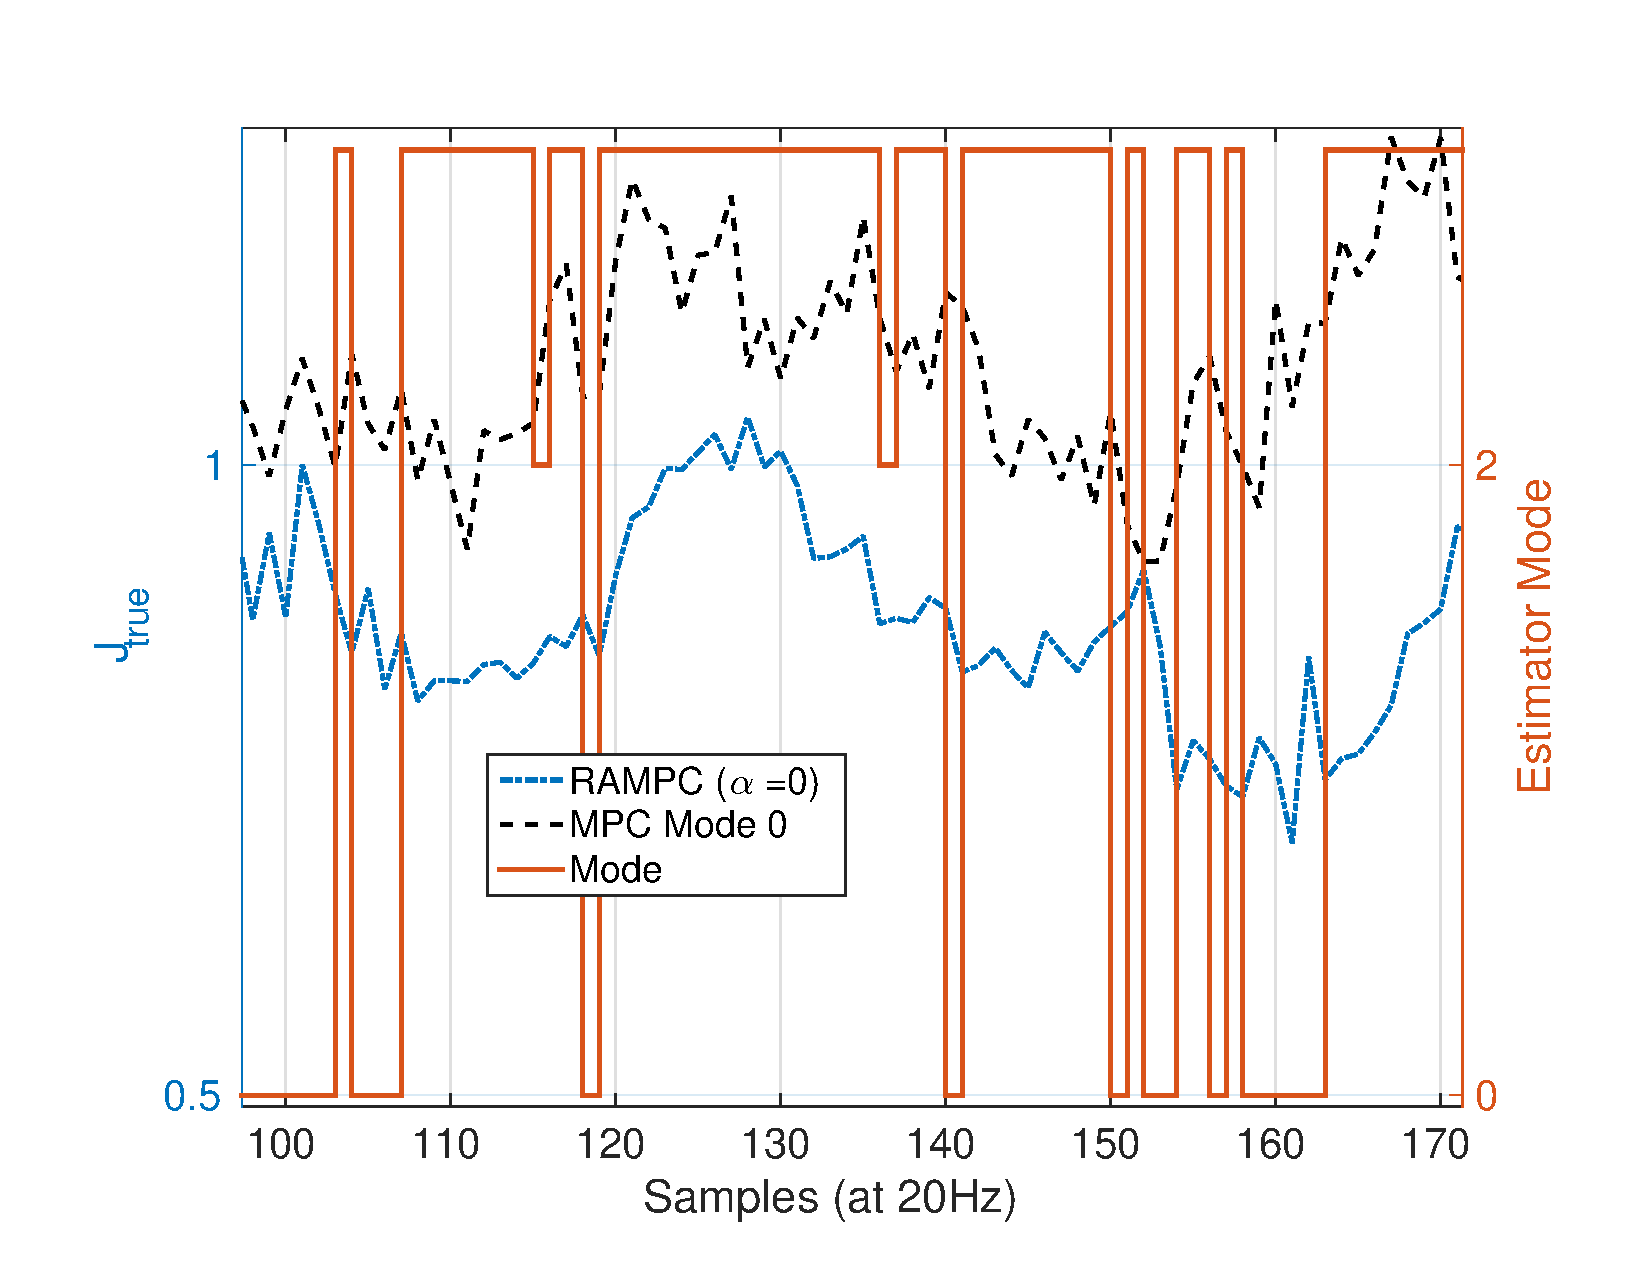
\includegraphics[width=0.49\textwidth]{figures/CostAndModes}
	\caption{Tracking cost at each time step for MPC (fixed mode 0 estimator) and RAMPC with $\alpha=0$. Note how the RAMPC performs better (lower cost) than the MPC and there is dynamic switching of estimator modes at runtime leading to improved performance for the RAMPC.}	
	\label{fig:CostAndModes}
\end{figure}


Figure \ref{fig:CostAndModes} shows how the tracking cost ($J_{true}$) evolves over time for RAMPC (with $\alpha=0$) and MPC (fixed mode 0) for a portion of the hexrotor flight. The estimator modes selected by RAMPC are overlaid in orange. Figure \ref{fig:CostAndModes} demonstrates that RAMPC has uniformly lower tracking cost than MPC, enabled by RAMPC's dynamic switching of estimator modes at runtime. Note that RAMPC exhibits better tracking performance throughout the flight and not just in this portion, and also outperforms MPC at other modes (see Table \ref{tbl:RAMPC_MPC_performance}).

Figure \ref{fig:TrackingVsEnergy} shows that RAMPC provides better tracking performance while using less energy to do so. For any fixed energy budget (a point on the x-axis), RAMPC delivers lower tracking cost (y-axis) than MPC. While MPC's tracking error is relatively constant across modes, RAMPC is able to balance tracking error with energy consumption by varying the $\alpha$ parameter. RAMPC's switching between estimation modes improves not only the control performance but also energy efficiency.


\begin{figure}[tbh]
	\centering
	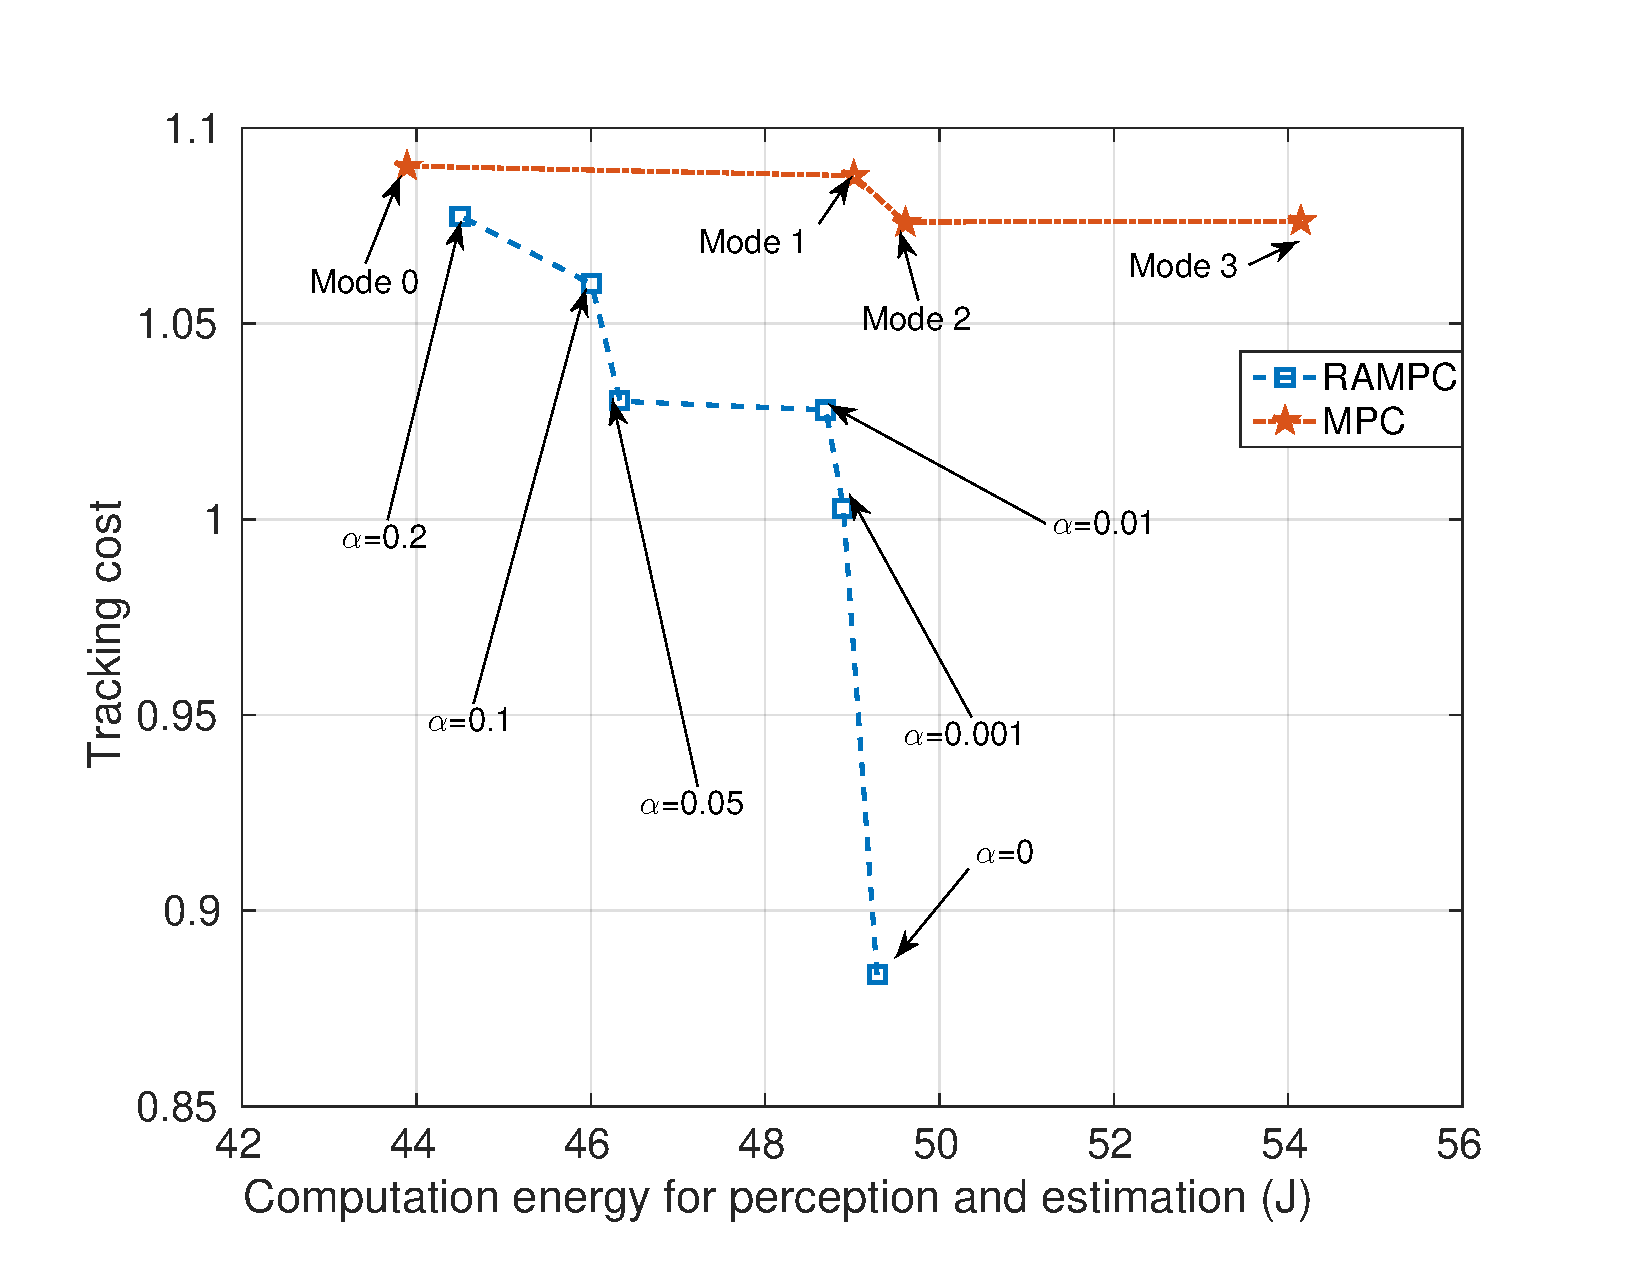
\includegraphics[width=0.49\textwidth]{figures/TrackingVsEnergy}
	\caption{Tracking cost vs estimated computation energy for executing the perception and estimation algorithm. Note for MPC, different energies are realized only by operating at different fixed modes of the perception and estimation algorithm. Using RAMPC as the controller, the different energies are due to run-time scheduling of different modes based on the optimal value of the cost function \ref{eq:tractableOptim} at each time step based on different values of $\alpha$. It is worth noting that RAMPC with co-design outperforms standard MPC on tracking performance across the entire range of energy consumption.}
	\label{fig:TrackingVsEnergy}
\end{figure}


\begin{table}[htb]
\begin{center}
\caption{Tracking performance and computation energy}
\label{tbl:RAMPC_MPC_performance}
\begin{tabular} {|c|c|c|c|c|}
	\hline
	\textbf{Controller} &\textbf{Est. Mode}/ $\pmb{\alpha}$ & $\pmb{E[J_{true}]}$ & $\pmb{\sigma({J_{true}})}$ & $\pmb{Energy(J)}$ \\ \hline
	MPC & 0/ $-$ & 1.0903 & 0.104 & 43.89\\ \hline
	MPC & 1/ $-$ & 1.0878 & 0.087 & 49.02 \\ \hline
	MPC & 2/ $-$ & 1.0760 & 0.098 & 49.60 \\ \hline
	MPC & 3/ $-$ & 1.0762 & 0.088 & 54.15 \\ \hline
	RAMPC &  $-$/0 & 0.8836 & 0.079 & 49.28 \\ \hline
	RAMPC & $-$/ 0.001 & 1.0029 & 0.093 & 48.90  \\ \hline
	RAMPC & $-$/ 0.01 & 1.0280 & 0.089 & 48.69  \\ \hline
	RAMPC & $-$/ 0.05 &1.0302 & 0.096 & 46.33 \\ \hline
	RAMPC & $-$/ 0.1 &1.0601 & 0.086 & 46.01 \\ \hline
	RAMPC & $-$/ 0.2 & 1.0776 & 0.083 & 44.49 \\ \hline
\end{tabular}	
	\end{center}
\end{table}



Figure \ref{fig:CostAndEnergyVsAlpha} shows the degradation (increased mean $J_{true}$) in tracking performance and reduction in energy consumption as the weight $\alpha$ for the computation power consumption in the cost function is increased. As energy becomes more important, RAMPC smoothly balances tracking cost and energy consumption. Table \ref{tbl:RAMPC_ModeTime} quantifies how RAMPC makes this trade-off, by showing the fraction of time spent in the 4 modes with RAMPC as $\alpha$ changes. While time is split between modes 0 and 3 with $\alpha=0$, more and more time is spent in the low-power (but less accurate) mode 0 as $\alpha$ increases.


\begin{figure}[t]
	\centering
	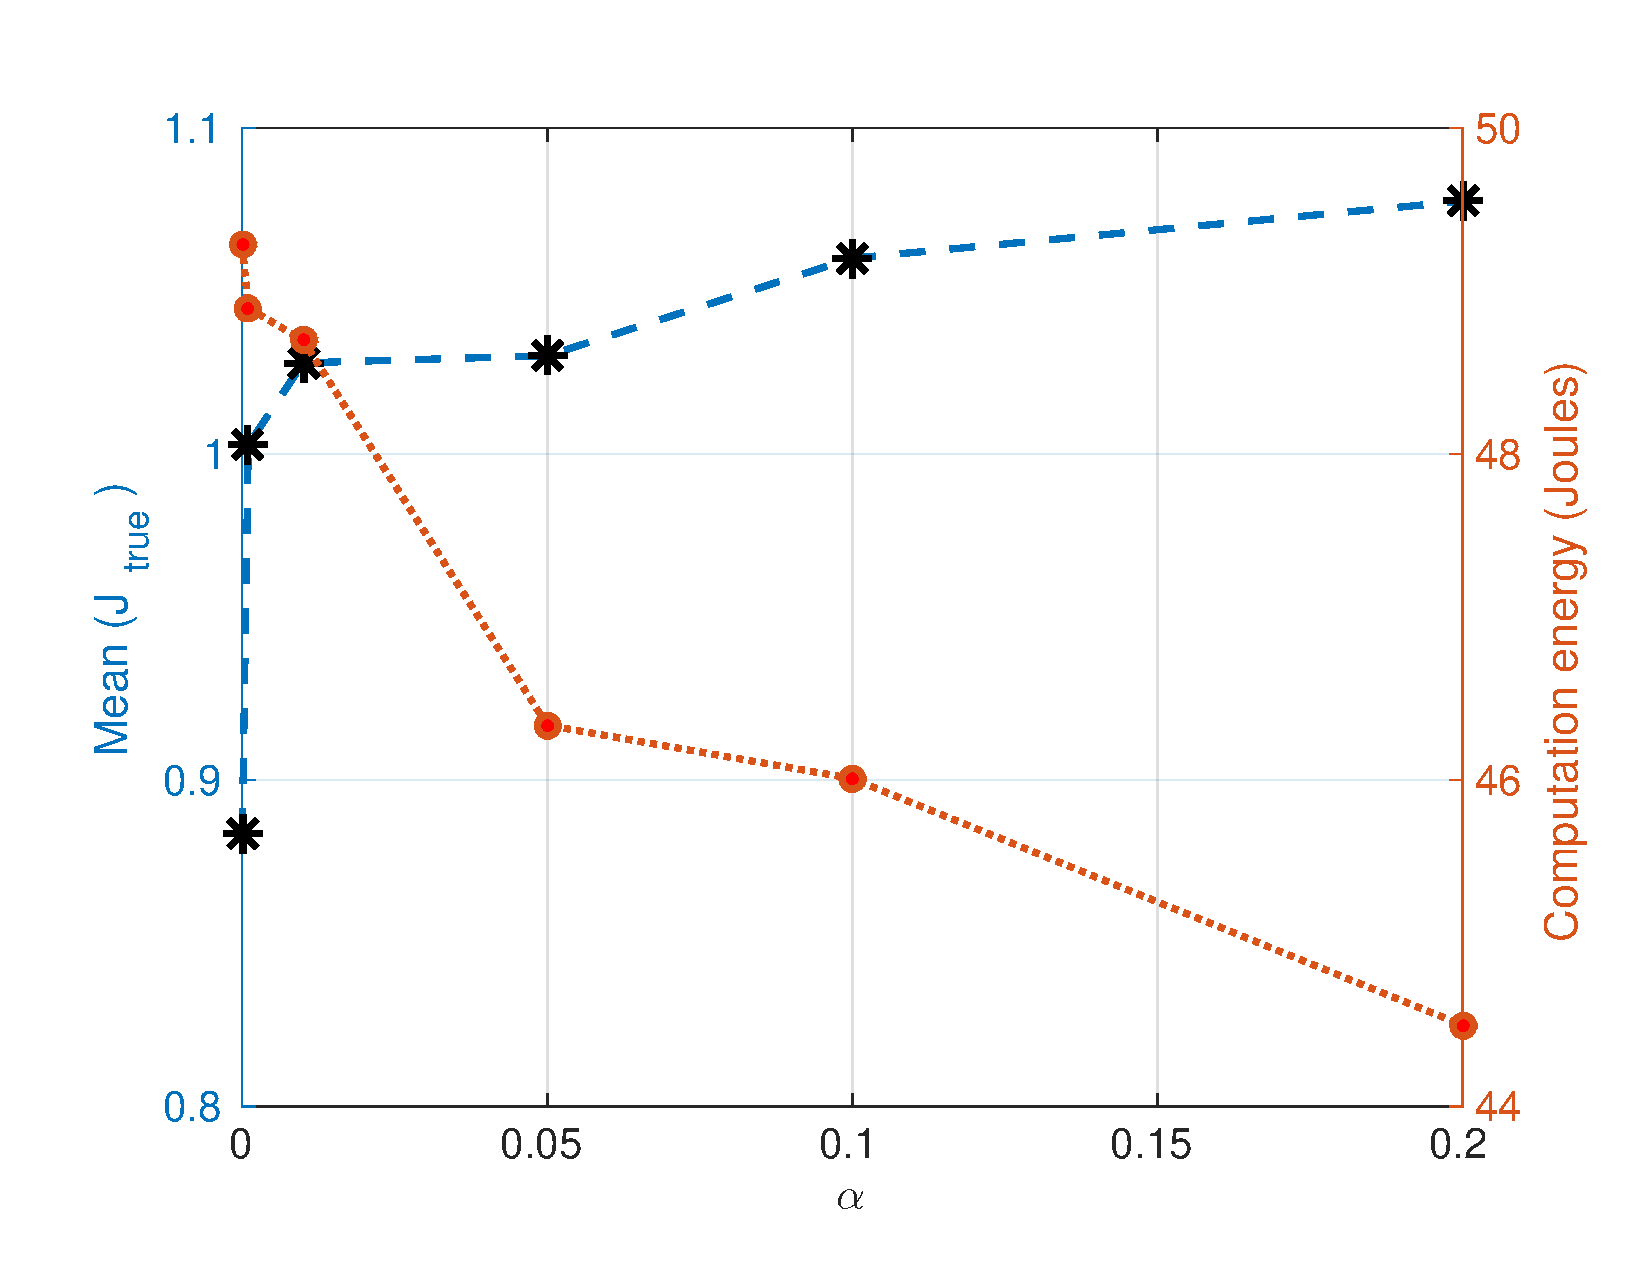
\includegraphics[width=0.49\textwidth,scale=0.7]{figures/CostAndEnergyVsAlpha}
        \vspace{-20pt}
	\caption{RAMPC tracking cost and estimated computation energy for the perception and estimation algorithm as a function of $\alpha$. }
	\label{fig:CostAndEnergyVsAlpha}
\end{figure}


\begin{table}[htb]
\begin{center}
\caption{Fraction of time spent in different estimator modes as $\alpha$ changes for RAMPC}
\label{tbl:RAMPC_ModeTime}
\begin{tabular} {|c|c|c|c|c|}
	\hline
	$\pmb{\alpha}$ & \textbf{Mode 0} & \textbf{Mode 1} & \textbf{Mode 2} & \textbf{Mode 3} \\ \hline
	0 & 0.461 & 0.009 & 0.020 & 0.510 \\ \hline
 	0.001 &  0.494 & 0.001 & 0.029 & 0.467 \\ \hline
	0.01 & 0.512 & 0.005 & 0.039 & 0.444  \\ \hline
	0.005 &  0.692 & 0.000 & 0.156 & 0.152 \\ \hline
	0.1 & 0.691 & 0.000 & 0.218 & 0.091 \\ \hline
	0.2 & 0.897 & 0.000 & 0.098 & 0.005  \\ \hline
	\end{tabular}	
	\end{center}
\end{table}

